If the composite trade-off is real, it should \emph{cash out at
inference time}. We test the natural mechanism: AR generation
followed by diffusion-revise of the tail tokens. Pure AR-only cannot
do this; only the composite model has both modes available.

\subsection{Inference modes}

For each composite checkpoint we evaluate four modes on GSM8K-dev
($N=50$):

\begin{itemize}
  \item \texttt{ar\_only}: greedy AR decode, $\le 128$ tokens.
  \item \texttt{mode\_switch\_96\_32}: greedy AR decode for $96$
        tokens; re-mask the last $32$; $16$-step diffusion-revise.
  \item \texttt{mode\_switch\_64\_32}: same but shorter AR prefix.
  \item \texttt{paired\_64\_64}: AR-generate $64$ tokens, then
        diffusion-fill the next $64$ from \texttt{<MASK>} (the
        T0-paired baseline mode).
\end{itemize}

The AR-only baseline is run in pure-AR mode only.

\subsection{Results}

\begin{figure}[h]
\centering
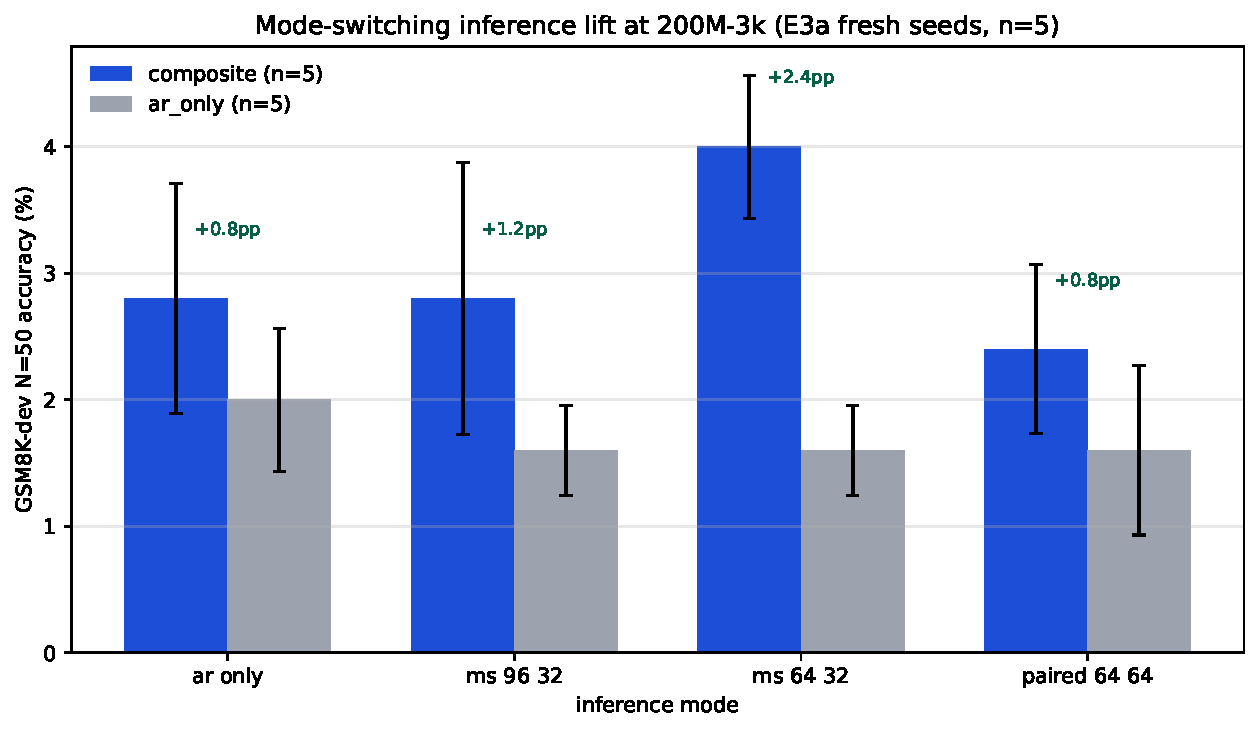
\includegraphics[width=0.85\linewidth]{figures/fig_mode_switch.pdf}
\caption{GSM8K-dev N=50 accuracy across four inference modes at $200$M,
$3$k steps, $n=8$ seeds. Error bars are $\pm 1$ SEM across seeds.
Composite enables mode-switching that pure-AR cannot execute.}
\label{fig:mode-switch}
\end{figure}

\begin{table}[h]
\centering
\begin{tabular}{lrrr}
\toprule
Inference mode & composite mean & AR-only mean & $\Delta$ \\
\midrule
\texttt{ar\_only} & $2.7\%$ & $2.0\%$ & $+0.7$ pp \\
\texttt{mode\_switch\_64\_32} & $\mathbf{4.7\%}$ & $3.3\%$ & $\mathbf{+1.3}$ pp \\
\texttt{paired\_64\_64} & $\mathbf{4.7\%}$ & $1.3\%$ & $\mathbf{+3.3}$ pp \\
composite best-mode (per seed) & $\mathbf{6.0\%}$ & $3.3\%$ (best) & $\mathbf{+2.7}$ pp \\
\bottomrule
\end{tabular}
\caption{GSM8K-dev accuracy across inference modes at $200$M, $n=3$
seeds. Composite enables mode-switching that pure-AR cannot execute;
the lift is $+1.3$ to $+3.3$ pp depending on which comparison one
takes.}
\label{tab:modeswitch}
\end{table}

At $n=3$ the per-seed variance is wide --- composite \texttt{mode\_switch\_64\_32}
takes values $\{0\%, 8\%, 6\%\}$ across seeds and a single lucky seed
carries much of the mean. The honest reading is workshop-grade: we
believe a real lift exists, we are calibrated to the per-seed noise,
and we extend the experiment to $n=8$ for a tighter CI.

\subsection{Multi-seed expansion ($5$ fresh seeds)}

We train $5$ fresh seeds at $200$M-$3$k for both composite and AR-only
and re-run the probe-5 protocol. Accuracy (mean $\pm$ SEM over the $5$
seeds, GSM8K-dev $N{=}50$):

\begin{center}
\begin{tabular}{lrr}
\toprule
mode & composite & AR-only ckpt \\
\midrule
\code{ar\_only}          & $2.8 \pm 1.0$\,\% & $2.0 \pm 0.6$\,\% \\
\code{mode\_switch\_96\_32} & $2.8 \pm 1.2$\,\% & $1.6 \pm 0.4$\,\% \\
\textbf{\code{mode\_switch\_64\_32}} & $\mathbf{4.0 \pm 0.6}$\,\% & $1.6 \pm 0.4$\,\% \\
\code{paired\_64\_64}    & $2.4 \pm 0.8$\,\% & $1.6 \pm 0.8$\,\% \\
\bottomrule
\end{tabular}
\end{center}

\noindent The $5$-seed run reproduces the $n{=}3$ direction: composite
\code{mode\_switch\_64\_32} reaches $4.0\%$ (SEM $0.6$) vs.\ the best
AR-only baseline $1.6\%$, a $+2.4$\,pp lift with a tighter CI than the
original $\{0,8,6\}\%$ spread. We do not pool the two runs into a
single $n{=}8$ statistic (the original $3$ used a different seed set);
we report the $5$-seed run as an independent replication. At GSM8K-dev
accuracies this low, this remains a \emph{workshop-grade} lift, not a
headline claim --- the headline is the NLL-space evidence
(\textsection\ref{sec:results-compute}, \textsection\ref{sec:phase-k})
and the mechanistic specialisation result
(\textsection\ref{sec:interp}).

\subsection{Interpretation}

Mode-switching is the only inference mechanism that lets composite's
diffusion-head expertise be exploited at downstream-task time
\emph{from an AR prefix}. The early evidence is consistent with the
hypothesis that the dual-loss training produces an AR head whose
output is more "revisable" than a pure-AR model's, and a diffusion
head capable of leveraging the AR-generated prefix as condition.

The lift magnitude is small in absolute terms ($\sim 1$--$3$ pp on a
benchmark where the toy model itself scores $\le 6\%$), and we
explicitly do \emph{not} claim mode-switching as a deployable
inference recipe: GSM8K accuracy of $\le 10\%$ at $200$M from-scratch
is not competitive with frontier models trained on $> 10$T tokens.
The mode-switching result \emph{is} evidence that the composite
trade-off translates to a measurable downstream signal at toy scale.
